\documentclass[11pt]{article}
\usepackage[utf8]{inputenc}
\usepackage{enumitem, xcolor, soul}
\sethlcolor{lightgray}
\usepackage{hyperref}
\usepackage{graphicx}

\usepackage[a4paper, margin=2.54cm]{geometry}

\pagestyle{empty}

\newcounter{Part}[section]
\newenvironment{Part}[1][]{\refstepcounter{Part}\par\medskip
   \noindent \large \textbf{Part~\thePart #1: }}{\medskip}



\begin{document}

% HEADER
\begin{flushleft}
    \rule[1mm]{\linewidth}{1.5pt} \\
    \large \textbf{Applied Epidemiology I: Spring 2021} \hfill \large Enoch Yi-Tung Chen \\
    \large  \textbf{Lab session using Stata}
    \hfill (enoch.yitung.chen@ki.se) \\
       \rule[1mm]{\linewidth}{1.5pt} \\
\end{flushleft}

\noindent \large{\textbf{Exercise 4}} \hfill \normalsize \textbf{15:15-16:45 (Mon.) 08 Feb, 2021}
\medskip

\noindent  Hi all, \\
This exercise 4 follows the lecture \textbf{Graphs}. However, you may also need to use some techniques from \textbf{Tables \& interpreting results} as well. You are expected to capture when to use graphs or tables to demonstrate your study results, and also how to plot graphs with sufficient information.

\medskip

\begin{Part}
\textbf{Types of graphs}
\end{Part}

\noindent Please open  your sphc\textunderscore all.dta and the codebook SPHC\textunderscore variable\textunderscore list.xls. 

\begin{enumerate}
	\item Make a \textbf{bar chart} to show how many participants joined the survey by year.
	\item Make a \textbf{box plot} to demonstrate overall self-rated health by year (or stratified by any variable if you would like).
	\item Following the question above, is box plot a good way to show the results here? Why or why not? (Hint: think about the definitions of median and mean. And what statistics is bar chart based on?)
	\item Following the question above, instead, how would you demonstrate the results? Try to write two sentences to describe your thought.
 \end{enumerate}

\begin{Part}
\textbf{twoway}
\end{Part}

\begin{figure}[h]
\begin{center}

	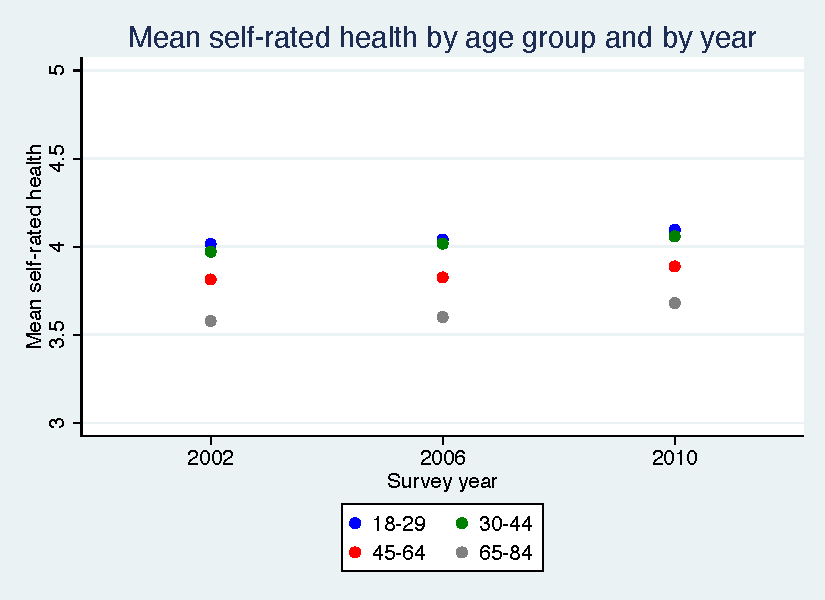
\includegraphics[scale=0.45]{images/mean_srh}
	\caption{Mean self-rated health by age group (18-29, 30-44, 45-64, 65-84) and by survey year (2002, 2006, 2010)}
		\end{center}

\end{figure}

\noindent Please plot "Mean self-rated health by age group, in 2002 2006 2010", similar to the figure above. \\
Suggested steps:
\begin{enumerate}
     \item Generate the mean of self-rated health by age group and by year. (Hint: \verb|tabstat|) 
     \item Put the statistics generated by \verb|tabstat| back to the dataset. (Hint: \verb|help tabstat|, \verb|return list|)
     \item Then plot a \textbf{scatter plot} showing mean self-rated health by age group and by year. (Hint: \verb|twoway scatter|) Think about why making a scatter plot instead of a line graph?
     \item[*] If you encounter difficulty in making this scatter plot, please at least try starting from Q2.3. Write some codes for the scatter plot, e.g., the legend, x-axis, y-axis, and titles.
     \end{enumerate}

\end{document}